\documentclass{llncs}
\usepackage[utf8]{inputenc}

\usepackage{alltt}
\usepackage{url}
\usepackage{graphicx}
\usepackage[percent]{overpic}

\usepackage{xcolor}
\DefineNamedColor{named}{cegla}         {rgb}{.81, .27, .13}
\newcommand{\al}[1]{\textcolor{Peach}{#1}}
\newcommand{\jp}[1]{\textcolor{cegla}{#1}}

\RequirePackage{pifont}
\newcommand{\cmark}{\ding{51}}

\usepackage{hyperref}

\newcommand{\typedliteral}{\textasciicircum\textasciicircum}
\newcommand{\protege}{\emph{Prot\'eg\'e}}


\title{An On-Line Learning to Query System}
\author{Jedrzej Potoniec}
\institute{Faculty of Computing, Poznan University of Technology\\ul. Piotrowo 3, 60-965 Poznan, Poland \\\email{Jedrzej.Potoniec@cs.put.poznan.pl}}

\sloppy

\begin{document}

\maketitle

\begin{abstract}
We present an on-line system which learns a SPARQL query from a set of wanted and a set of unwanted results of the query.
The sets are extended during a dialog with the user.
The system leverages SPARQL 1.1 and does not depend on any particular RDF graph.
\end{abstract}

\section{Introduction}

A common problem with querying a Linked Data dataset is that the user must have prior knowledge about the vocabulary used by the dataset.
If a user is already familiar with the dataset this is a minor inconvenience, but for a user who is new to the dataset the learning curve may be really steep, to the point that the user decides not to use the dataset at all.
A typical approach to remedy the problem is to use some tool helping the user to formulate a SPARQL \cite{Harris:13:SQL} query, using e.g. faceted browsing \cite{DBLP:conf/semweb/Ferre14a}, natural-language interfaces  \cite{hoffner2016survey}, visual interfaces \cite{DBLP:conf/semweb/ZainabSMZDH15} or recommendations \cite{DBLP:conf/semweb/Campinas14}.
In all these system the user specifies the query by various means.
We propose a different approach, where the user only specifies what should and what should not be in the results of the query, and the system takes care of formulating the query.
The user does not need to know SPARQL, it is enough for her to be able to distinguish wanted and unwanted results.
The system operates by conducting a dialog with the user.
In each part of the dialog, the user is asked about a small set of URIs and for every URI she must decide if it should or should not be present in the results of the final query.
A similar approach was already presented in  \cite{DBLP:conf/esws/LehmannB11}, where the system used mostly computational power of the computer system of the user.
We leverage new features of SPARQL 1.1 and move most of the computation to a SPARQL endpoint.

Thought this work, we use the following prefixes: \texttt{dbr:} for \url{http://dbpedia.org/resource/}, \texttt{dbo:} for \url{http://dbpedia.org/ontology/}, \texttt{dbp:} for \url{http://dbpedia.org/property/}, \texttt{dct:} for \url{http://purl.org/dc/terms/}, \texttt{xsd:} for \url{http://www.w3.org/2001/XMLSchema#}.

\section{System Description}



A screenshot of the on-line system is presented in \autoref{fig:sc1}.
The backend of the system was developed in \emph{Python 3} with \emph{RDFlib}\footnote{\url{https://github.com/RDFLib/rdflib}} and the frontend uses \emph{Bootstrap}\footnote{\url{http://getbootstrap.com/}} and \emph{JQuery}\footnote{\url{http://jquery.com/}}.
Integration between the backend and the frontend is done using \emph{Pycnic}\footnote{\url{http://pycnic.nullism.com/}}, a \emph{Python} library for developing JSON APIs.
The source code of the system is available in a \emph{Git}\footnote{\url{https://git-scm.com/}} repository available at \url{https://bitbucket.org/jpotoniec/kretr/}.
An instance of the system is available at \url{https://semantic.cs.put.poznan.pl/ltq/}.
It uses a SPARQL endpoint set up on \emph{Blazegraph\footnote{\url{https://www.blazegraph.com/}} 2.1.1} and loaded with \emph{DBpedia 2015-04}.
Note that the system itself does not depend neither on \emph{Blazegraph} nor \emph{DBpedia}, as it can use any SPARQL 1.1 endpoint.


\begin{figure}
\centering
%\includegraphics[width=\textwidth]{sc1.png}
\begin{overpic}[width=\textwidth,tics=10]{ltq.png} %grid,
  \put (40,55) {\huge 1}
  \put (90,55) {\huge 2}
  \put (27,5) {\huge 3a}
  \put (87,5) {\huge 3b}
  \put (80,20) {\huge 4}
  \put (35,17) {\huge 5}
\end{overpic}
\caption{
A screenshot of the system while the user is supposed to assign new examples to correct sets.
The view is divided into six areas: new examples, which are to be assigned (1), the current query (2), the URIs already assigned by the user: wanted (3a) and unwanted (3b), a form to add a new URI by hand (4) and demo scenarios (5).
}
\label{fig:sc1}
\end{figure}

The aim of the system is to build a SPARQL SELECT query with a single variable in the head.
The variable has a modifier DISTINCT.
The query contains only a WHERE clause (i.e. there is no GROUP BY, ORDER BY etc.), and in the clause there is only a basic graph pattern (BGP, i.e. triple patterns and filter expressions).
The undirected graph corresponding to the BGP is a connected graph and the filter expressions are of form \emph{variable \texttt{>=/<=} literal}.
An example of such a query is
\begin{alltt}
SELECT DISTINCT ?uri
WHERE \{
    ?uri dct:subject dbr:Category:City_counties_of_Poland .
    ?uri dbo:populationTotal ?anon1.
    FILTER(?anon1 >= "205934"^^xsd:nonNegativeInteger). \}
\end{alltt}

\begin{figure}
\centering
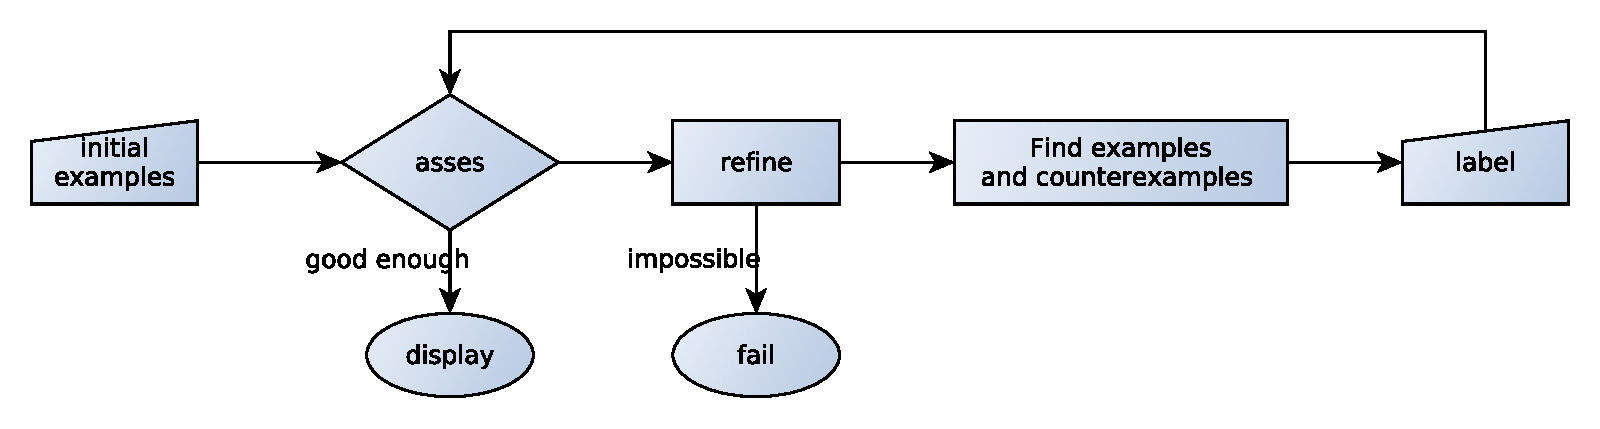
\includegraphics[width=\textwidth]{diagram.pdf}
\caption{A typical workflow with the system.
First the user specifies a small set of examples, then the system works in a loop: asses a hypothesis, refines it, finds new examples and asks the user to decide about them.
}
\label{fig:workflow}
\end{figure}

A typical workflow with the system is presented in \autoref{fig:workflow}.
First, the user specifies a small set of URIs that should be present in the results of the final query, and a small set of URIs that should not be present in the results.
Then, the system poses a few queries to the SPARQL endpoint to compute a possible query that is consistent with the set specified by the user.
The consistency is verified using a well-known information retrieval metrics: \emph{recall} and \emph{$F_1$ measure}.
The query is then used to find a few new examples that are in the results of the query and next few examples that are not in the results.
In each case we require the found examples to be new, i.e. they must not already be labeled by the user.
The user is then asked to decide about each example if it should or not be present in the results of the final query (i.e. the user extends the sets defined in the beginning).
After the user decides, the system checks if the decisions agrees with the query.
If they do not,  the cycle repeats: the system refines the query, asks the user and assess the query.
Otherwise, the system assumes that the correct query was found.
The query is displayed to the user along with the results of the query.
If the user decides that the results are not satisfactory, she must add at least one new URI to one of the sets.




\section{Proposed Demo}

During the demo, we will present to the participants how to use the system, what types of queries are possible to learn and what are the limitations.
The system has embedded two demo scenarios: the first one to find a query to select all capitals of the member states of European Union and the second one to find a query to select all Polish cities having more than $200'000$ citizens.
For the presentation, we will use the on-line instance available at \url{https://semantic.cs.put.poznan.pl/ltq/}.

\section{Conclusion}

In this paper we presented a system which is able to learn a SPARQL query from two sets of URIs obtained from the user in a dialog.
The system leverages new features of SPARQL 1.1 and does not depend on any particular RDF graph.
It also does not require any precomputation before it is ready to use.
The source code is publicly available.

\subsubsection*{\ackname}
Jedrzej Potoniec acknowledges the support from the Polish National Science Center (Grant No 2013/11/N/ST6/03065).


\bibliographystyle{splncs03}
\bibliography{main}


\end{document}
